\documentclass{article} % For LaTeX2e
\usepackage{nips15submit_e,times}
\usepackage{hyperref}
\usepackage{url}
\usepackage{amsmath,amsfonts,amsthm,amssymb,pgf,tikz}
\usepackage{color}
\usepackage[mathscr]{euscript}
%\usepackage{wrapfig}
%\usepackage{subfigure}
\usepackage{graphicx} % more modern
\usepackage{subfigure}
\usepackage{enumerate}
%\documentstyle[nips14submit_09,times,art10]{article} % For LaTeX 2.09


\title{PPAML Team Challenge Problem Proposal}


\author{
a \\
\texttt{a@berkeley.edu} \\
\And
Coauthor \\
Affiliation \\
Address \\
\texttt{email} \\
\AND
Coauthor \\
Affiliation \\
Address \\
\texttt{email} \\
}

% The \author macro works with any number of authors. There are two commands
% used to separate the names and addresses of multiple authors: \And and \AND.
%
% Using \And between authors leaves it to \LaTeX{} to determine where to break
% the lines. Using \AND forces a linebreak at that point. So, if \LaTeX{}
% puts 3 of 4 authors names on the first line, and the last on the second
% line, try using \AND instead of \And before the third author name.

\newcommand{\fix}{\marginpar{FIX}}
\newcommand{\new}{\marginpar{NEW}}

\nipsfinalcopy % Uncomment for camera-ready version

\begin{document}


\maketitle

\section{Problem Description and Justification}
\newcommand{\secref}[1]{Section~\ref{#1}}
\newcommand{\figref}[1]{Figure~\ref{#1}}
\newcommand{\tabref}[1]{Table~\ref{#1}}
\renewcommand{\eqref}[1]{Equation~(\ref{#1})}

\newcommand{\mbf}[1]{\mbox{{\bf #1}}}
\newcommand{\shortcite}{\cite}
\newcommand{\smbf}[1]{\mbox{{\scriptsize\bf #1}}}
\def\w{\mbf{w}}

%\section{Introduction}
%% {\centering\scriptsize\em
%%   Substantial portions of this text are reproduced from an
%%   author's paper~\cite{friedman1997image}.}

{\bf Foreground/Background Video Segmentation:}
Recognizing and tracking moving
objects is one of the main uses of vision.
For computer vision, we can start with `merely' identifying the
foreground.
%first identify what part of each
%frame is due to moving objects.
%(subsequently, separating and tracking
%individuals across frames are also important subproblems)
That is, the task here is to decompose
each frame of video into two parts: all of the moving objects, and
everything else.  Thankfully, in practice, approximate answers are
good enough.  \secref{sec:formal-problem} formally defines the problem,
but first, some background.

For many years, the ``obvious'' approach has
been first to compute some stationary {\em background image}, and then to
identify the moving objects as those pixels in each frame that
differ significantly from the background. We will call this the
{\em background subtraction} approach.
The details of the method are described briefly in
\secref{background-subtraction-section}.

To pick one application, the Roadwatch project at Berkeley,
background subtraction is overall an effective means of
locating and tracking moving vehicles in freeway
traffic~\cite{Koller+al:1994}.
However, in some important cases, background subtraction performs
poorly at vehicle detection: long shadows and heavy traffic.
Shadows move, but treating them as real parts of the vehicles they
overlap leads to many problems, starting with reliably separating each
vehicle from one another.
Moreover, background subtraction tends to treat any
sufficiently slowly changing pixel as
background, which is a problem in heavy traffic because vehicles
then too often disappear into the background.\footnote{Interestingly,
  many natural predators are also only able to see movement, so that
  freezing in place grants invisibility.}

These problems are not specific to freeway monitoring, as they arise
from the oversimplified view of the
general task---detecting moving objects---that
background subtraction takes.  Namely, the approach assumes that
background never changes and foreground always changes.  However,
occasionally-variable background and occasionally-constant
foreground are also possible.  Handling those, when important, needs a
more sophisticated approach; probabilistic techniques prove useful in practice,
especially the use of Expectation-Maximization (EM)~\cite{Dempster+al:1977}.

There is a large literature (several hundred papers in the last
decade, and several annual conferences) on the application
of EM and its family of closely related techniques
to image reconstruction, image segmentation, and
motion identification.   Applications include optical astronomy, laser
range finders, synthetic aperture radar, magnetic resonance imaging, PET, microscopy, and
X-rays.  Almost without exception, EM is used to identify classes of
pixels within an image or classes of motions within an optical flow
field, on the assumption that similar pixels can be grouped
together. Typical examples include Samadani~\cite{Samadani:1995},
Jepson and Black~\cite{Jepson+Black:1993}, Sawhney and
Ayer~\cite{Sawhney+Ayer:1996}, and Weiss and
Adelson~\cite{Weiss+Adelson:1996}.

\subsection{PPAML Motivation}

Interestingly, even just using a simple three-class (``background'', ``darkened'',
``occluded'') mixture model already significantly improves upon
background subtraction for the Roadwatch application~\cite{friedman1997image}.  See
\secref{shadow-and-background-subtraction-section} for a summary of
that approach---which we take as baseline.

This baseline is interesting firstly because it is a natural
probabilistic generalization of the 
classical deterministic approach.
Secondly and more importantly of interest, significant further
improvement should be possible, for example `just' developing and
applying a more complicated probabilistic model should work.

We note, however, that getting inference to work on our suggested baseline
model, on the real application, was not a small amount of
implementation effort.  That severely limited the scope of alternative models we could
feasibly investigate at that time.  A useful probabilistic programming
system would allow a much broader investigation into possible models,
by automating away some of the work presently required when working
from a language with little to no special support for probability.


\subsubsection{Reuse and Tuning}

We expect any implementation to `work' on any video input, although
the quality of the segmentation may be abysmal when core assumptions are
challenged.  For example, the baseline---and background
subtraction---critically assumes a stationary camera.  A moving camera
will provoke nonsense.

Besides that, while motivated from freeway
traffic, the baseline model and accompanying implementation  make few assumptions.
For example, the model does not assume that all shadows have to point
the same way.  We could have exploited that, and it would have yielded
better segmentations on freeway traffic data.  Since we did not build in any such assumption about light
sources, we expect that our model will perform the same at
identifying and ignoring shadows regardless of the number or geometry of light sources.

We hope that
any effort implementors do put into optimizing for some specific
assumptions about the kinds of videos that will be seen is easily
adapted to work well for other situations.  Patient-monitoring in
hospitals and facial-recognition at airports are two such potential applications
where one might expect a foreground-detector trained on freeway data
to still function reasonably well without further massive tuning/training.
It would be interesting to see the results of such cross-domain
application.  How much incremental work is needed by each PPS/team to get
acceptable results as noncritical assumptions change?


\subsubsection{Modularity}

As demonstrated by the existing work,
reasonably effective performance on the problem is easy enough to
achieve without relying on large, preexisting, machine vision
implementations.  That is helpful for those probabilistic programming
systems that limit callouts to other runtimes.

At the same time, getting the segmentation nearly as correct as a
human in every case has roughly the same structure as presently typical
CAPTCHAs (picking out objects in sufficiently complicated images and
videos is considered human-feasible but computer-infeasible).
If aiming for that or similarly high
levels of performance, then a PPS that permits reuse of
preexisting implementations could easily demonstrate a significant
advantage.


\subsubsection{Space Efficiency}

Video data is an interesting stress test of a PPS.  What is the
overhead the system accrues when representing distributions over
datastructures?  Likely too much by default, since uncompressed video
can be large
enough to stress test even deterministic languages.  It will be
interesting to see what answers each PPS provides for working with
models too big to entirely fit in memory all at once.  Is the effort
required to control the PPS's memory overhead more, or less, than the
effort required to implement probability theory in a deterministic
language?



%% To pick two
%% potential flaws of the reference work: it fails to consider nighttime
%% and deliberately ignores contiguity.
%% Much like shadows, the pixels brightened
%% by vehicles' headlights are easily misclassified as real parts of the
%% vehicles.  Using four classes
%% (``background'', ``brightened'', ``darkened'', ``occluded'') could help.
%% The reference work can be confused by a gray vehicle driving over a
%% gray manhole: it can mistakenly imagine that the manhole remains
%% visible when the vehicle drives over it.  Adding probabilistic contiguity
%% constraints would combat that and many related potential flaws.





%\subsection{Notation}
%\label{sec:notation}


\subsection{Foreground Video Segmentation}
\label{sec:formal-problem}

The goal is to take an input video and select a subset of each
frame---ideally in real-time---corresponding to whatever the notion of
``interesting'' is.  The selection of a subset of each frame is a
\emph{segmentation} of the original video; the selected subset is the
\emph{foreground} and its complement is the \emph{background}, the two
together are the segmentation of the frame.

Concretely, there are all sorts of hairy details to decide upon about the
precise representation, storage, and transmisison of input videos and
segmentations. In the online/real-time setting there are further details to
decide upon, in particular, limits on maximum 
and average latency (is 1 second too long?).

Abstractly, a video can be represented as a function $I(x,y,t)$ giving
the value at time $t$ of the pixel at $(x,y)$.  The frames will be
rectangular and fixed 
size, so $x$ is in some set $\{0,1,\ldots,n\}$ and $y$ is in another
$\{0,1,\ldots,m\}$.  The framerate will be constant, and so the domain
of time is just $\{0,1,\ldots,T\}$.  The nature of pixel values
(grayscale, RGB, HSV, CMYK, \ldots) will be specified and constant
(probably red, green, blue).

A segmentation can be represented as a mask, that is, as a function
$M(x,y,t)$ onto either 0 or 1.  ``1'' means ``interesting''; so
$M(150,60,70)=0$ is the assertion that, at time $70$, the pixel at
$(150,60)$ is background according to segmentation $M$.

It is often very useful, even necessary, to process video
\emph{online}, which here means to pick the segmentation of the
current frame in some bounded amount of time.  In that setting we
can emphasize time by writing $I_t(x,y)=I(x,y,t)$
for the current frame (the one at time $t$) and $M_t(x,y)=M(x,y,t)$
for its segmentation.  A typical constraint on such algorithms is to
compute an answer using only some bounded memory of the past: each
$M_t$ should depend on only $I_{t-k},\ldots, I_t$ for some $k$.

``Interesting'' will not be given an entirely formal
definition; intuitively, the interesting things are the things that
move.  But as mentioned, there are application-specific exceptions: a
stopped vehicle is interesting, a shadow is not.
A (partially?) labeled training set will exemplify the notion for
whatever source of video is chosen.
So the overall task is to both learn the concept (offline), and
predict it (ideally online).

A fully labeled training set is just some distinguished set of videos and
corresponding segmentations, usually somewhat imperfect:
$\{(I,M) \mid \text{$M$ is (probably, approximately) a correct
  segmentation of $I$}\}$ is the form of a training set.

The precise notion of quality of prediction will be specified, but in
practice the most appropriate definition varies wildly.  Ideally each
PPS will be able to easily adjust its behavior to suit a wide range of
plausible performance metrics.





%% Some systems/participants may want to communicate their uncertainty
%% about the interesting subset of each frame.  That is difficult to---and
%% we will not---accomodate, as there are too many ways to be uncertain.  For example,
%% our baseline would prefer to assign a probability to each pixel
%% (rather than 0/1).  Other approaches might want to consider spatial
%% dependencies, for example by presenting a (perhaps weighted) set of
%% sampled frames.  Still others might want to report a symbolic
%% representation of a distribution over the present frame.  The truly
%% ambituous consider also temporal dependencies (by working with
%% distributions over whole segmentations).

%% For evaluation purposes, we settle on the simplest thing, which is to
%% demand a single (most likely) estimate of each frame in turn.  Each
%% will then be scored by its distance to the notionally correct answer,
%% where ``distance'' will be some well-specified metric on frames (such
%% as ``number of correct foreground pixels'').  The
%% scores for each frame will then be aggregated in some specified
%% fashion (averaging, maxing, or something more exotic).
%% There is no
%% way to reach consensus on the best possible scoring or aggregation
%% functions (or even that the score of a segmentation should be any form
%% of aggregration of per-frame scores); any particular application has
%% its own peculiar set of consequences for being wrong.\footnote{It would be
%% better, for example, to optimize the probability of identifying any
%% fatal threat rather than to optimize the accuracy of ones estimate of
%% the total number of moving objects.}

%% An interesting meta-evaluation is to assess how easily each 
%% implementation can be adapted if the performance metric is changed.
%% Is the language flexible enough to explicitly model not only the
%% question, but also the full metric over wrong answers?



\section{Feasibility}

The baseline implementation was made without support from a dedicated
probabilistic programming system.  So it is certainly feasible for any
team to implement a solution.  One could just ignore the special
nature of a PPS---treat it like a deterministic language---and just repeat
the prior work.

As for us, our language and supporting implementation were designed specifically
to aid redoing and improving the particular application of video segmentation to
freeway data as well as to aid the many other real-world
applications of probability that our principal investigator has worked
on.

Particularly BLOG's declarative format 
is meant to permit rapid investigation of differing models without
having to spend any significant time, especially human time, on
customizing the inference strategy/implementation to the model.  That
is, in our experience, both in general and on the particular task of
segmenting video, iterating on the model chosen is usually much more
effective than `fussing' with the details of the implementation of
inference. 

To contrast, procedural languages
shine when the right model is relatively obvious, but large or
otherwise difficult to solve. Chess, for example, is easy to model but hard to
solve.  Many real-world applications, including video segmentation,
have the entirely opposite character of being difficult to model well,
but, once found, good enough models are easy enough to solve.


\paragraph{Data}
Any publicly available video feed from a stationary camera is enough
to get started, and there are plenty of those.  If publishing
recordings of humans runs into legal troubles, it would be enough to,
for example, point a camera at an acquarium and make the task be one
of detecting fish.\footnote{Detecting fish raises an interesting
  computational point
  not encountered in freeway traffic data: if plants and currents are
  boring, then 
  a plant moving due to 
  current is still boring.  Conversely, if plants are interesting,
  then even never-moving plants are still ``foreground''.}
The only tricky thing with video is that it is usually far too
time-consuming to have a human label every pixel of an entire video.
That primarily raises questions about the nature and reproduciblity of
evaluation.  It becomes a data availability issue when the test itself
is kept secret, and there are several scenarios where that is
desirable or necessary.


%% There are several standard workarounds, each with problems.  One is to have an
%% independent judge pick some tiny fraction of the possible test
%% questions.  That is, pick some
%% interesting and tiny subset of contestant-unseen pixels, label them,
%% and score the contestants for their labels of just those pixels.  It
%% is easy to skew the results by careful selection, which is why the
%% independence of the judge is important.  It is also difficult to ever
%% reproduce the full challenge.  If the test questions and labels are
%% kept secret, then reproducibility is immediately out the window.  If
%% published after the competition, then the scores can be independently
%% verified, but the full nature of the challenge cannot be repeated
%% (since absence of foreknowledge of the test questions is key to making
%% this an interesting way to evaluate systems).

%% Another workaround is to generate synthetic data, so that ground truth
%% is known with absolute certainty.  The standard complaint is that it
%% is easy to generate synthetic data that is too clean, or noisy in the
%% wrong way.

%% Yet another workaround is to pick one particular system as the gold
%% standard, its only flaw being that executing it is usually
%% prohibitively costly.  (Humans as experts could be viewed as a limiting case of
%% `too expensive to execute'.)  One avenue we are considering is to use
%% Robust PCA as the gold standard; the submitted solutions then have to
%% demonstrate some substantial computational advantage over that method.

\paragraph{Risks}
There are no obvious significant risks.
It should be easy to settle the details such that running this
challenge only has the systems passively observing and quietly
inferring; taking no action besides using up
electricity should presumably be considered to have no serious risks.\footnote{The paranoid can imagine a fire breaking out in a server room during,
and perhaps partially due to, the computation.  Bleeding hearts can
agonize over the possibility that the massive computation is the last
straw that pushes a major city into a sustained brownout, during which
electrically-dependent humans would die.}
Implausibly, if---to obtain
labeled traffic data---one instruments many drivers and set them to
driving they would not otherwise be doing, then there are risks and
liability concerns should two collide.  (But there is no reason to
insist upon traffic data in the first place.)



\section{Evaluation}
\begin{enumerate}[i]
\item The solution of this problem should provided 0/1 labels for each pixel in every frame of the test videos. Label 0 denotes this pixel represents the background in the current frame while label 1 denotes the foreground. We could measure the accuracy of the provided solution by comparing every predicted label against the ground truth of the test videos. A successful solution should provide prediction results should be no worse than the incremental EM solution in \cite{friedman1997image}.
    Moreover, the solution provided by the teams must be online. In order to predict the result, we also need to evaluate the running time to produce labels for a single frame comparing against the total running time. The processing time for each frame for a successful online solution should be roughly the total time divided by the number of frames.
\item In prior work we implemented a form of online expectation
  maximization as inference for a natural probabilistic
  generalization of background subtraction\cite{friedman1997image}.
  (The \emph{model} is a natural 
  generalization; the inference is significantly more
  complicated than taking an average over frames.)  The following two sections
  reproduce that paper's description of background subtraction and our
  generalization of it.
\item There are many existing background substraction datasets. We could use a renderer engine to generate some small synthetic data as well as use a real-world dataset, i.e. the UCSD dataset\footnote{\url{http://www.svcl.ucsd.edu/projects/background_subtraction/ucsdbgsub_dataset.htm}}, for evaluating the performance.
\item The teams should load the video frames from disk and output all the labels for each video frame in a single text file. For example, when the video name is \texttt{A}, then the result for the 1st frame in \texttt{A} should be stored in \texttt{A1.txt}. The evaluation script should load all the labels from the text files and evaluate the predicted accuracy.
\item In the first stage, we will only deliver the small synthetic data. In the second stage, we deliver a small portion of the UCSD dataset to the teams and evaluate the performance using the remaining videos. Another choice for the second stage could be that for each video data in the UCSD dataset, we deliver only the first 25\% to the teams and using the whole video (or the remaining 75\%) for evaluation.
\end{enumerate}



\subsection{Background Subtraction}
\label{background-subtraction-section}

{\em\centering This and the following section is an excerpt from prior
  work~\cite{friedman1997image}.}

The roots of background subtraction go back to the 19th century, when
it was shown that the background image could be obtained simply by
exposing a film for a period of time much longer than the time
required for moving objects to traverse the field of view. Thus, in
its simplest form, the background image is the long-term average
image:
\[ B(x,y,t) = \frac{1}{t}\sum_{t'=1}^t I(x,y,t') \]
where $I(x,y,t)$ is the instantaneous pixel value for the $(x,y)$
pixel at time $t$. This can also be computed incrementally:
\[B(x,y,t) = \frac{(t-1)}{t}B(x,y,t-1) + \frac{1}{t}I(x,y,t)\]
The variance can also be computed incrementally, and moving
objects can be identified by thresholding the Mahalanobis distance
between $I(x,y,t)$ and $B(x,y,t)$.

One obvious problem with this approach is that lighting conditions
change over time. This can be handled using a moving-window average,
or, more efficiently, using exponential forgetting. In the latter
scheme, each image's contribution to the background image is weighted
so as to decrease exponentially as it recedes into the past. This is
implemented by the update equation
\begin{equation}
B(x,y,t) = (1-\alpha)B(x,y,t-1) + \alpha I(x,y,t)
\label{forgetting-equation}
\end{equation}
where $1/\alpha$ is the time constant of the forgetting process.
Unlike the moving-window method, this requires no additional storage.
Exponential forgetting is equivalent to using a Kalman filter to track
the background image, as done in~\cite{Koller+al:1994}.




\begin{figure*}[t]
\centering
\subfigure[a]{

\includegraphics[width=0.31\textwidth]{figures/avg.0099.ps}
}
\subfigure[b]{
\includegraphics[width=0.31\textwidth]{figures/img.0100.ps}
}
\subfigure[c]{
\includegraphics[width=0.31\textwidth]{figures/mask.0100.ps}
}
\caption{(a) Background image computed during fast-moving traffic
using exponential forgetting. (b) Current image (frame 100). (c) Thresholded
difference image showing pixels associated with moving objects.}
\label{fast-traffic-figure}
\end{figure*}

\figref{fast-traffic-figure} shows a typical result from the method
operating under favourable conditions. Although there are a few stray
pixels identified as ``moving'' due to image noise, the vehicles are
outlined reasonably well. Standard methods can be used to group the
pixels belonging to each vehicle and to compute and track a smoothed
convex hull.

The sharp-eyed reader will have spotted that the background
subtraction method succeeds not only in detecting moving vehicles, but
also their shadows.\footnote{Some of the road markings are also
labelled as ``moving''---this is due to camera jitter.
Also, the method fails to detect those parts of a moving vehicle that
are approximately the same intensity as the background.
Such problems are unavoidable in any pixel-based method.}
In practice, shadows have been one of the most
serious problems for video-based traffic surveillance in both
commercial and research systems~\cite{Michalopoulos:1991}, sometimes
resulting in undercounting or overcounting by as much as 50\%.  It
might be thought that some simple fix such as lightening or
thresholding might work to eliminate shadows, but these schemes may fail
because parts of the road may be shadowed by buildings, and because of
road markings---a shadow falling on a white line can still result in a
brighter pixel than sunlight falling on tarmac~\cite{Kilger:1992}.

As mentioned in the introduction, another serious problem arises when
objects are slow-moving or temporarily stationary. Here, ``slow-moving''
means that the time of
traversal is non-negligible compared with $1/\alpha$,
the time constant of the exponential forgetting process in
\eqref{forgetting-equation}. When this happens,
the background image becomes corrupted and object detection fails
completely (\figref{slow-traffic-figure}).

\begin{figure*}[t]
\subfigure[a]{
\includegraphics[width=0.31\textwidth]{figures/avg.0924.ps}
}
\subfigure[b]{
\includegraphics[width=0.31\textwidth]{figures/img.0925.ps}
}
\subfigure[c]{
\includegraphics[width=0.31\textwidth]{figures/mask.0925.ps}
}
\caption{(a) Background image computed during slow-moving traffic
using exponential forgetting. (b) Current image (frame 925). (c) Thresholded
difference image showing pixels associated with moving objects.}
\label{slow-traffic-figure}
\end{figure*}

As it turns out, a solution to both difficulties is to first
\emph{classify} and then \emph{selectively update}.  Roughly, only
updating the background image with those pixels presently classified as
belonging to it gives better results.  There are stable and
unstable ways to go about the selective updating; the stable way
hinges on a properly Bayesian treatment of the classification of the
pixels.  In other words, we define a generative
probabilistic model of pixel values given pixel classes; subsequently
the math fully determines, by Bayes Rule, the optimal classification
given observed values.  In practice the implementation must
cut some corners for the sake of feasibility, the details of that are
in the original paper~\cite{friedman1997image}. 


\subsection{Probabilistic Shadow and Background Subtraction}
\label{shadow-and-background-subtraction-section}
\label{pixel-model-section}


Consider a single pixel and the distribution of its values over time.
Some of the time it will be in its ``normal'' background state---for
example, a small area of the road surface. Some of the time it may be
in the shadow of moving vehicles, and some of the time it may be part
of a vehicle. Thus, in the case of traffic surveillance, we can think
of the distribution of values $i_{x,y}$ of a pixel $(x,y)$ as the
weighted sum of three distributions $r_{x,y}$ (road), $s_{x,y}$
(shadow), and $v_{x,y}$ (vehicle):
\[ i_{x,y} = \w_{x,y} \cdot (r_{x,y},\ s_{x,y},\ v_{x,y}) \]
These distributions are subscripted
to emphasize that they differ from pixel to pixel; $r_{x,y}$ is a
probability distribution for the way that {\em this specific pixel}
looks when it is showing unshadowed road at the corresponding physical
location. It is essential to have different models for each pixels,
because, for example, some parts of the image may correspond to white road
markings, others to dark streaks in the centers of lanes, and still
others to lamp-posts (see \figref{fast-traffic-figure}).
The weights are also subscripted, because some pixels
may spend more time in shadow or vehicle than others.

\begin{figure*}[t]
\subfigure[a]{
\includegraphics[width=0.23\textwidth]{graphs/intensity-freq.ps}
}
\subfigure[a]{
\includegraphics[width=0.23\textwidth]{graphs/rgb-scatter.ps}
}
\subfigure[a]{
\includegraphics[width=0.23\textwidth]{graphs/intensity-model.ps}
}
\subfigure[a]{
\includegraphics[width=0.23\textwidth]{graphs/rgb-model.ps}
}
\caption{(a) Empirical distribution of intensity values for pixel (160,170)
over 1000 frames. (b) Scatter plot of RGB values for the same pixel.
(c) Fitted three-component Gaussian mixture model for the data in (a).
(d) Scatter plot of 1000 randomly-generated data points from a fitted
three-component Gaussian mixture model for the data in (b).}
\label{pixel-model-figure}
\end{figure*}

Figures~\ref{pixel-model-figure}(a) and~\ref{pixel-model-figure}(b)
show the empirical distribution of intensity and RGB values,
respectively, for pixel (160,170), which is roughly two-thirds of the
way towards the bottom right corner of the image.  These data display
the behaviour one would expect: the shadow and road pixels form two
fairly well-defined peaks, while the vehicle pixels are widely
scattered.  As a first approximation, we assume that each distribution
can be modelled as a Gaussian.  Using expectation maximization, we can fit three-component mixture models to the
data. \figref{pixel-model-figure}(c) shows the fitted model for
intensity values, and \figref{pixel-model-figure}(d) shows a scatter
plot for the fitted RGB model. The fitted models are reasonably good
(but far from ideal) approximations to the empirical data.

%the techniques described in
%\secref{EM-section},
%%
%% the label problem solution is in {results-section}
%%

The model for pixel $(x,y)$ is parameterized by the parameters $\Theta
= \{
w_l, \mu_l, \Sigma_l : l \in \{ r, s, v \}\}$ so that $\w_{x,y} = (w_r,
w_s, w_v )$, $r_{x,y} \sim N(\mu_r,\Sigma_r)$, and so on.%
\footnote{For clarity, we omit the subscript $x,y$ from the names of
these parameters. However, it should be clear that there is a
different set of parameters for pixel position $x,y$.}
Our models apply in two settings. In the first, we examine intensity
levels, and $\mu$ and $\Sigma$ are scalars. In the second, we examine
RGB values, and $\mu$ is a $3\times 1$ vector and $\Sigma$ is a $3\times 3$
matrix. The derivations are identical in the two cases, so we do not
distinguish between them in the following discussion.

Let $i$ be a pixel value (either an intensity level or a vector of RGB
values). Let $L$ be a random variable denoting the {\em label\/} of
the pixel in this image. Our model defines the probability that $L =
l$ and $I(x,y,t) = i$ to be
\begin{eqnarray*}
\lefteqn{P( L = l, I(x,y,t) = i \mid \Theta ) = {}} \\
 & &  w_l \cdot
(2\pi)^{-\frac{d}{2}}|\Sigma_l|^{-\frac{1}{2}} \exp\{-\frac{1}{2}(i -
\mu_l)^T {\Sigma_l}^{-1} (i - \mu_l)\}
\end{eqnarray*}
where $d$ is the dimension of each pixel value (1 or 3 in our case).
Given these probabilities, we can classify the pixel value. Namely, we
choose the class $l$ with highest posterior  probability $P( L = l \mid I(x,y,t)) $.


\section{Dissemination}
\begin{enumerate}[i]
\item All the algorithms and data could be published. Hence, any people could re-produce the result by re-implementing the algorithm in some PPS.
\item There could be new models and now tools for the online background substraction problem. The problem itself is very important for real-world applications.
\end{enumerate} 

\section{Suggested Reviewers}
We suggest Vikash Mansinghka and Noah Goodman to review the proposal since they have related experiences in image processing problems. 


{\small
\bibliography{BIB/references}
\bibliographystyle{abbrv}
}

\end{document}
